
% !TEX program = pdflatex
\documentclass[aspectratio=169,10pt]{beamer}

\usetheme{Madrid}
\usecolortheme{default}
\setbeamertemplate{navigation symbols}{}
\setbeamertemplate{caption}[numbered]
\usefonttheme{professionalfonts}

\usepackage{amsmath,amssymb,bm,mathtools}
\usepackage{graphicx}
\usepackage{booktabs,tabularx,array}
\usepackage{siunitx}
\usepackage{tikz}
\usepackage{pgfplots}
\usepackage[american,siunitx]{circuitikz}
\pgfplotsset{compat=1.18}
\usetikzlibrary{arrows.meta,positioning,calc,patterns}

\usepackage[most]{tcolorbox}
\usepackage{listings}
\usepackage{xcolor}

\graphicspath{{Figures/}}

\lstdefinelanguage{Matlab}{
  keywords={break,case,catch,continue,else,elseif,end,for,function,global,if,otherwise,persistent,return,switch,try,while},
  morekeywords={expm,ss,c2d,ode45,zeros,ones,size,disp,clear,clc,eye,diag,eig},
  sensitive=true,
  morecomment=[l]\%,
  morestring=[m]'
}
\lstset{
  language=Matlab,
  basicstyle=\ttfamily\scriptsize,
  keywordstyle=\color{blue!70!black}\bfseries,
  commentstyle=\color{green!40!black},
  stringstyle=\color{orange!70!black},
  numbers=left,
  numberstyle=\tiny\color{gray!70},
  numbersep=6pt,
  showstringspaces=false,
  breaklines=true,
  frame=single,
  rulecolor=\color{gray!40}
}

\tcbset{
  beamer,
  enhanced,
  colback=white,
  colframe=blue!60!black,
  boxrule=0.6pt,
  arc=2pt,
  left=5pt,right=5pt,top=4pt,bottom=4pt
}
\newtcolorbox{defnbox}[1]{title=#1, colframe=blue!70!black, colback=blue!3}
\newtcolorbox{notebox}[1]{title=#1, colframe=teal!70!black, colback=teal!3}
\newtcolorbox{examplebox}[1]{title=#1, colframe=orange!80!black, colback=orange!3}
\newtcolorbox{alertbox}[1]{title=#1, colframe=red!75!black, colback=red!4}

\newcommand{\R}{\mathbb{R}}
\newcommand{\T}{^\top}
\newcommand{\dd}{\,\mathrm{d}}

\title[State-Space Representation]{State-Space Representation of Dynamic Systems}
\subtitle{MSc Model Predictive Control}
\author{Dr Ibrahim Kucukdemiral}
\institute{Glasgow Caledonian University}
\date{\today}

\begin{document}

\begin{frame}
\titlepage
\end{frame}

\begin{frame}{A guiding thought}
\begin{quote}
\itshape
``The sciences do not try to explain, they hardly even try to interpret, they mainly make models.
By a model is meant a mathematical construct which, with the addition of certain verbal interpretations,
describes observed phenomena.''
\end{quote}
\hfill --- \textbf{John von Neumann}
\end{frame}

\section{Introduction}

\begin{frame}{Why this chapter matters for MPC}
The quality of any MPC controller depends directly on the quality of the prediction model.
To predict future trajectories and optimise future inputs, we need a mathematical representation that is:
\begin{itemize}
  \item accurate enough to capture the relevant dynamics,
  \item structured enough to analyse,
  \item efficient enough for real-time computation.
\end{itemize}

In practice:
\begin{itemize}
  \item physical systems are \textbf{continuous-time},
  \item many systems are \textbf{nonlinear},
  \item controllers are implemented \textbf{digitally},
  \item many standard MPC formulations rely on \textbf{linear discrete-time models}.
\end{itemize}

\begin{notebox}{Flow of ideas}
Physics \(\rightarrow\) state-space model \(\rightarrow\) equilibrium \(\rightarrow\) linearisation \(\rightarrow\) discretisation \(\rightarrow\) MPC prediction model.
\end{notebox}
\end{frame}

\begin{frame}{What we cover in this chapter}
\begin{itemize}
  \item A short review of continuous-time state-space models.
  \item Practical derivation of models for mechanical and electrical systems.
  \item Physical interpretation of states.
  \item Equilibrium points and operating points.
  \item Local linearisation of nonlinear systems using Taylor expansion and Jacobians.
  \item Exact discretisation of continuous-time LTI systems using the matrix exponential.
  \item Discretisation of forced LTI systems under Zero-Order Hold (ZOH).
  \item Numerical discretisation of nonlinear systems using Forward Euler and RK4.
  \item Stability of discrete-time systems in the \(z\)-plane and via Lyapunov/Stein equations.
\end{itemize}
\end{frame}

\section{What is state-space?}

\begin{frame}{What is state-space, and why is it central to MPC?}
State-space modelling describes a dynamic system using a set of \textbf{internal variables} called states.

\begin{defnbox}{Central principle}
If the state \(x(t)\) is known at a given time, and the future inputs are known, then the future behaviour of the system is determined.
\end{defnbox}

This is exactly the property required by MPC:
\begin{itemize}
  \item the controller measures or estimates the current state,
  \item predicts future states and outputs,
  \item computes an optimal future input sequence.
\end{itemize}
\end{frame}

\begin{frame}{General nonlinear continuous-time state-space model}
A general nonlinear continuous-time state-space model is written as
\[
\dot{x}(t)=f\big(x(t),u(t),t\big),
\qquad
y(t)=h\big(x(t),u(t),t\big).
\]

Here:
\begin{itemize}
  \item \(x(t)\in\R^n\): state vector,
  \item \(u(t)\in\R^m\): input vector,
  \item \(y(t)\in\R^p\): output vector,
  \item \(f(\cdot)\): dynamics map,
  \item \(h(\cdot)\): output map.
\end{itemize}

\begin{notebox}{Interpretation}
This compact vector form is simply a structured way of writing \(n\) coupled first-order differential equations.
\end{notebox}
\end{frame}

\begin{frame}{Expanded state equation}
\[
\underbrace{
\begin{bmatrix}
\dot{x}_1(t)\\
\dot{x}_2(t)\\
\vdots\\
\dot{x}_n(t)
\end{bmatrix}}_{\dot{x}(t)}
=
\underbrace{
\begin{bmatrix}
f_1(x_1,\dots,x_n,u_1,\dots,u_m,t)\\
f_2(x_1,\dots,x_n,u_1,\dots,u_m,t)\\
\vdots\\
f_n(x_1,\dots,x_n,u_1,\dots,u_m,t)
\end{bmatrix}}_{f(x(t),u(t),t)}
\]

\begin{itemize}
  \item \(x_i(t)\): the \(i\)-th state,
  \item \(u_j(t)\): the \(j\)-th input,
  \item \(f_i(\cdot)\): the \(i\)-th differential equation.
\end{itemize}
\end{frame}

\begin{frame}{Expanded output equation}
\[
\underbrace{
\begin{bmatrix}
y_1(t)\\
y_2(t)\\
\vdots\\
y_p(t)
\end{bmatrix}}_{y(t)}
=
\underbrace{
\begin{bmatrix}
h_1(x_1,\dots,x_n,u_1,\dots,u_m,t)\\
h_2(x_1,\dots,x_n,u_1,\dots,u_m,t)\\
\vdots\\
h_p(x_1,\dots,x_n,u_1,\dots,u_m,t)
\end{bmatrix}}_{h(x(t),u(t),t)}
\]

Outputs are the measurable or externally visible quantities.
They need not be the full state vector.
\end{frame}

\begin{frame}{Linear Time-Invariant (LTI) state-space form}
For linear time-invariant systems, the model simplifies to
\begin{align*}
\dot{x}(t) &= A x(t) + B u(t),\\
y(t) &= C x(t) + D u(t).
\end{align*}

The matrices have clear roles:
\begin{itemize}
  \item \(A\): internal dynamics,
  \item \(B\): input-to-state coupling,
  \item \(C\): state-to-output mapping,
  \item \(D\): direct feedthrough.
\end{itemize}

\begin{notebox}{Why this matters in MPC}
LTI models are especially attractive because they lead naturally to efficient linear-algebraic predictions and convex optimisation problems.
\end{notebox}
\end{frame}

\begin{frame}{Physical interpretation of states}
In practice, states are usually chosen from variables associated with stored energy or internal configuration:
\begin{itemize}
  \item \textbf{Electrical systems:} currents in inductors, voltages across capacitors,
  \item \textbf{Mechanical systems:} positions and velocities,
  \item \textbf{Process systems:} temperatures, pressures, concentrations.
\end{itemize}

These choices are natural because the governing physical laws are differential equations in these variables.

\begin{notebox}{Important caveat}
We may also intentionally introduce additional states, such as:
\begin{itemize}
  \item integral states,
  \item disturbance estimates,
  \item bias states.
\end{itemize}
These are not necessarily physical, but they are extremely useful in control design.
\end{notebox}
\end{frame}

\begin{frame}{Why state-space is so useful in MPC}
The importance of state-space in MPC can be summarised as follows:
\begin{itemize}
  \item \textbf{Recursive prediction:} the model can be propagated forward step by step.
  \item \textbf{Natural MIMO description:} multi-input multi-output systems are handled directly through matrices.
  \item \textbf{Direct constraint handling:} bounds on states and inputs can be expressed algebraically.
  \item \textbf{Systematic discretisation:} continuous-time physics can be converted into discrete-time prediction equations.
\end{itemize}

\begin{alertbox}{Bottom line}
State-space is the modelling language that links physical intuition, mathematical analysis, and predictive control design.
\end{alertbox}
\end{frame}

\section{Modelling from physical laws}

\begin{frame}{Example: nonlinear modelling of a simple pendulum}
\begin{columns}[T,totalwidth=\textwidth]
\begin{column}{0.42\textwidth}
\begin{center}
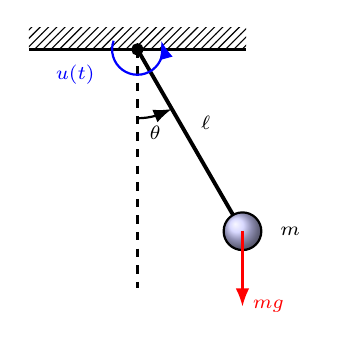
\begin{tikzpicture}[thick, >=Latex, scale=0.92]
  \fill [pattern = north east lines] (-1.5,0) rectangle (1.5,0.3);
  \draw (-1.5,0) -- (1.5,0);
  \filldraw [black] (0,0) circle (2pt);
  \draw [dashed] (0,0) -- (0,-3.3);
  \draw [line width=1.4pt] (0,0) -- (1.45,-2.51) node [midway, above right] {\scriptsize $\ell$};
  \shade [ball color=blue!20] (1.45,-2.51) circle (0.26);
  \draw (1.45,-2.51) circle (0.26) node [right=0.35cm] {\scriptsize $m$};
  \draw [->] (0,-0.95) arc (270:300:0.95) node [midway, below] {\scriptsize $\theta$};
  \draw [->, red] (1.45,-2.51) -- (1.45,-3.55) node [right] {\scriptsize $mg$};
  \draw [->, blue, domain=160:380] plot ({0.35*cos(\x)}, {0.35*sin(\x)});
  \node [blue, left] at (-0.45,-0.35) {\scriptsize $u(t)$};
\end{tikzpicture}
\end{center}
\end{column}
\begin{column}{0.58\textwidth}
Apply rotational Newton's law:
\[
\tau_{\text{net}} = I\ddot{\theta},\qquad I=m\ell^2.
\]

Torques acting on the pendulum:
\begin{itemize}
  \item control torque: \(+u(t)\),
  \item gravity: \(-mg\ell\sin\theta\),
  \item viscous damping: \(-b\dot{\theta}\).
\end{itemize}

Hence
\[
m\ell^2 \ddot{\theta}=u(t)-mg\ell\sin\theta-b\dot{\theta},
\]
so
\[
\ddot{\theta}=
-\frac{g}{\ell}\sin\theta
-\frac{b}{m\ell^2}\dot{\theta}
+\frac{1}{m\ell^2}u(t).
\]
\end{column}
\end{columns}
\end{frame}

\begin{frame}{Pendulum: nonlinear state-space form}
Choose the states
\[
x_1(t)=\theta(t),\qquad x_2(t)=\dot{\theta}(t).
\]

Then
\begin{align*}
\dot{x}_1 &= x_2,\\
\dot{x}_2 &= -\frac{g}{\ell}\sin(x_1)-\frac{b}{m\ell^2}x_2+\frac{1}{m\ell^2}u.
\end{align*}

Therefore
\[
\dot{x}=
\begin{bmatrix}
x_2\\[4pt]
-\dfrac{g}{\ell}\sin(x_1)-\dfrac{b}{m\ell^2}x_2+\dfrac{1}{m\ell^2}u
\end{bmatrix}.
\]

If the output is the angle,
\[
y=\begin{bmatrix}1 & 0\end{bmatrix}x = x_1.
\]

\begin{notebox}{Observation}
This is a nonlinear state-space model because of the \(\sin(x_1)\) term.
\end{notebox}
\end{frame}

\begin{frame}{Pendulum: small-angle linearisation}
Near \(\theta=0\), use the small-angle approximation
\[
\sin(\theta)\approx \theta.
\]

Then the model becomes
\begin{align*}
\dot{x}_1 &= x_2,\\
\dot{x}_2 &= -\frac{g}{\ell}x_1-\frac{b}{m\ell^2}x_2+\frac{1}{m\ell^2}u.
\end{align*}

Hence
\[
\dot{x}=Ax+Bu,
\]
with
\[
A=
\begin{bmatrix}
0 & 1\\[4pt]
-\dfrac{g}{\ell} & -\dfrac{b}{m\ell^2}
\end{bmatrix},
\qquad
B=
\begin{bmatrix}
0\\[4pt]
\dfrac{1}{m\ell^2}
\end{bmatrix}.
\]

The output equation remains
\[
y=Cx+Du,\qquad
C=\begin{bmatrix}1 & 0\end{bmatrix},\quad D=\begin{bmatrix}0\end{bmatrix}.
\]
\end{frame}

\begin{frame}{Example: state-space modelling of an RLC circuit}
Choose
\[
x_1=i_L,\qquad x_2=v_C,\qquad u=v_i.
\]

\begin{center}
\begin{circuitikz}[scale=0.75]
  \draw (2, 5) to[sinusoidal voltage source, l={$V_i$}] (2, 9);
  \draw (2, 9) to[american resistor, l={$R_1$}] (5, 9);
  \node[circ] at (5, 9){};
  \draw (5, 9) to[cute inductor, l={$L$}] (5, 5);
  \draw (5, 9) to[american resistor, l={$R_2$}] (8, 9);
  \node[circ] at (8, 9){};
  \draw (8, 9) to[capacitor, l={$C$}] (8, 5);
  \node[circ] at (5, 5){};
  \draw (8, 5) -- (5, 5) -- (2, 5);
  \node[ground] at (5, 5){};
  \draw[-Latex] (4.75, 8.5) -- (4.75, 7.5);
  \node at (4.25,7.95) {\scriptsize $i_L$};
  \node at (5.25,9.45) {\scriptsize $v_L$};
  \node at (8.25,9.45) {\scriptsize $v_C$};
\end{circuitikz}
\end{center}

Constitutive relations:
\[
v_L = L\frac{\dd i_L}{\dd t},
\qquad
i_C = C\frac{\dd v_C}{\dd t}.
\]
\end{frame}

\begin{frame}{RLC circuit: derivation of the state equations}
Current through \(R_2\):
\[
i_{R_2} = \frac{v_L-v_C}{R_2}.
\]

Applying KCL at the capacitor node:
\[
C\dot{v}_C = \frac{v_L-v_C}{R_2}.
\]

Applying KCL at the inductor node:
\[
\frac{v_i-v_L}{R_1}=i_L+\frac{v_L-v_C}{R_2}.
\]

Solving for \(v_L\):
\[
v_L=
\frac{R_2}{R_1+R_2}v_i
-\frac{R_1R_2}{R_1+R_2}i_L
+\frac{R_1}{R_1+R_2}v_C.
\]
\end{frame}

\begin{frame}{RLC circuit: final state-space form}
Substituting into the element equations gives
\begin{align*}
\dot{i}_L &=
-\frac{R_1R_2}{L(R_1+R_2)}i_L
+\frac{R_1}{L(R_1+R_2)}v_C
+\frac{R_2}{L(R_1+R_2)}v_i,\\[4pt]
\dot{v}_C &=
-\frac{R_1}{C(R_1+R_2)}i_L
-\frac{1}{C(R_1+R_2)}v_C
+\frac{1}{C(R_1+R_2)}v_i.
\end{align*}

Thus with \(x=[\,i_L\;\;v_C\,]\T\),
\[
\dot{x}=Ax+Bu,
\]
where
\[
A=
\begin{bmatrix}
-\dfrac{R_1R_2}{L(R_1+R_2)} & \dfrac{R_1}{L(R_1+R_2)}\\[8pt]
-\dfrac{R_1}{C(R_1+R_2)} & -\dfrac{1}{C(R_1+R_2)}
\end{bmatrix},
\qquad
B=
\begin{bmatrix}
\dfrac{R_2}{L(R_1+R_2)}\\[8pt]
\dfrac{1}{C(R_1+R_2)}
\end{bmatrix}.
\]
\end{frame}

\begin{frame}{Example: mass--spring--damper system}
Equation of motion:
\[
m\ddot{\zeta}(t)+c\dot{\zeta}(t)+k\zeta(t)=F(t).
\]

Choose
\[
x_1=\zeta,\qquad x_2=\dot{\zeta},\qquad u=F(t).
\]

Then
\begin{align*}
\dot{x}_1 &= x_2,\\
\dot{x}_2 &= -\frac{k}{m}x_1-\frac{c}{m}x_2+\frac{1}{m}u.
\end{align*}

Hence
\[
\dot{x}=Ax+Bu,
\]
with
\[
A=
\begin{bmatrix}
0 & 1\\[4pt]
-\dfrac{k}{m} & -\dfrac{c}{m}
\end{bmatrix},
\qquad
B=
\begin{bmatrix}
0\\[4pt]
\dfrac{1}{m}
\end{bmatrix}.
\]

If \(y=\zeta=x_1\), then
\[
y=Cx+Du,\qquad
C=\begin{bmatrix}1 & 0\end{bmatrix},\quad D=\begin{bmatrix}0\end{bmatrix}.
\]
\end{frame}

\section{Nonlinear systems and local linearisation}

\begin{frame}{Why nonlinear systems matter}
Many practical systems are nonlinear.
Examples of nonlinearities include:
\begin{itemize}
  \item trigonometric geometry,
  \item saturation and dead-zones,
  \item aerodynamic drag,
  \item nonlinear stiffness,
  \item friction effects,
  \item chemical reaction kinetics.
\end{itemize}

A general nonlinear model is
\begin{align*}
\dot{x}(t) &= f(x(t),u(t)),\\
y(t) &= h(x(t),u(t)).
\end{align*}

Unlike linear systems, nonlinear systems:
\begin{itemize}
  \item may have multiple equilibria,
  \item are not governed by superposition,
  \item can behave very differently at different operating points.
\end{itemize}
\end{frame}

\begin{frame}{Equilibrium points}
An equilibrium is a state of operation where the system ceases to evolve.

\begin{defnbox}{Continuous-time equilibrium}
For \(\dot{x}=f(x,u)\), a pair \((x_e,u_e)\) is an equilibrium if
\[
f(x_e,u_e)=0.
\]
\end{defnbox}

\begin{defnbox}{Discrete-time equilibrium}
For \(x_{k+1}=f(x_k,u_k)\), a pair \((x_e,u_e)\) is an equilibrium if
\[
x_e = f(x_e,u_e).
\]
\end{defnbox}
\end{frame}

\begin{frame}{Physical interpretation of equilibria}
Equilibria are also called:
\begin{itemize}
  \item steady states,
  \item operating points,
  \item trim points.
\end{itemize}

Examples:
\begin{itemize}
  \item \textbf{Mechanical:} rest or constant-velocity motion,
  \item \textbf{Electrical:} constant DC currents and voltages,
  \item \textbf{Thermal/process:} balanced inflows and outflows so that variables remain constant.
\end{itemize}

In control, we usually want the closed-loop system to converge to a desired equilibrium.
\end{frame}

\begin{frame}{Scalar Taylor expansion about an equilibrium}
Consider the scalar nonlinear system
\[
\dot{x}=f(x,u),
\]
and let \((x_e,u_e)\) be an equilibrium.

The first-order Taylor approximation about \((x_e,u_e)\) is
\[
f(x,u)\approx f(x_e,u_e)
+\frac{\partial f}{\partial x}\Big|_{(x_e,u_e)}(x-x_e)
+\frac{\partial f}{\partial u}\Big|_{(x_e,u_e)}(u-u_e).
\]

Since \(f(x_e,u_e)=0\),
\[
\dot{x}\approx
\frac{\partial f}{\partial x}\Big|_{(x_e,u_e)}(x-x_e)
+
\frac{\partial f}{\partial u}\Big|_{(x_e,u_e)}(u-u_e).
\]
\end{frame}

\begin{frame}{Multivariable Jacobian linearisation}
For the vector system
\[
\dot{x}=f(x,u),\qquad x\in\R^n,\quad u\in\R^m,
\]
the linearised model about \((x_e,u_e)\) is
\[
\dot{x}\approx A(x-x_e)+B(u-u_e),
\]
where
\[
A=\left.\frac{\partial f}{\partial x}\right|_{(x_e,u_e)},
\qquad
B=\left.\frac{\partial f}{\partial u}\right|_{(x_e,u_e)}.
\]

Defining deviation variables
\[
\tilde{x}=x-x_e,\qquad \tilde{u}=u-u_e,
\]
gives
\[
\dot{\tilde{x}}=A\tilde{x}+B\tilde{u}.
\]
\end{frame}

\begin{frame}{Output linearisation}
If the output map is nonlinear,
\[
y=h(x,u),
\]
then its first-order expansion about \((x_e,u_e)\) gives
\[
\tilde{y}=C\tilde{x}+D\tilde{u},
\]
where
\[
C=\left.\frac{\partial h}{\partial x}\right|_{(x_e,u_e)},
\qquad
D=\left.\frac{\partial h}{\partial u}\right|_{(x_e,u_e)}.
\]

Thus the full linearised model is
\begin{align*}
\dot{\tilde{x}} &= A\tilde{x}+B\tilde{u},\\
\tilde{y} &= C\tilde{x}+D\tilde{u}.
\end{align*}
\end{frame}

\begin{frame}{Example: planar duorotor nonlinear model}
Choose
\[
x=
\begin{bmatrix}
p_x & p_y & \theta & \dot{p}_x & \dot{p}_y & \dot{\theta}
\end{bmatrix}\T,
\qquad
u=
\begin{bmatrix}
u_1\\u_2
\end{bmatrix}.
\]

Nonlinear dynamics:
\begin{align*}
m\ddot{p}_x &= -(u_1+u_2)\sin(\theta),\\
m\ddot{p}_y &= (u_1+u_2)\cos(\theta)-mg,\\
J\ddot{\theta} &= \frac{\ell}{2}(u_2-u_1).
\end{align*}

Equivalent first-order form:
\begin{align*}
\dot{x}_1 &= x_4, &
\dot{x}_2 &= x_5, &
\dot{x}_3 &= x_6,\\
\dot{x}_4 &= -\frac{1}{m}(u_1+u_2)\sin x_3, &
\dot{x}_5 &= \frac{1}{m}(u_1+u_2)\cos x_3 - g, &
\dot{x}_6 &= \frac{\ell}{2J}(u_2-u_1).
\end{align*}
\end{frame}

\begin{frame}{Planar duorotor: equilibrium and linearised model}
At hover,
\[
x_e=
\begin{bmatrix}
0&0&0&0&0&0
\end{bmatrix}\T,
\qquad
u_{1,e}=u_{2,e}=\frac{mg}{2}.
\]

Linearising about hover gives
\[
\dot{\tilde{x}}=A\tilde{x}+B\tilde{u},
\]
with
\[
A=
\begin{bmatrix}
0 & 0 & 0 & 1 & 0 & 0\\
0 & 0 & 0 & 0 & 1 & 0\\
0 & 0 & 0 & 0 & 0 & 1\\
0 & 0 & -g & 0 & 0 & 0\\
0 & 0 & 0 & 0 & 0 & 0\\
0 & 0 & 0 & 0 & 0 & 0
\end{bmatrix},
\quad
B=
\begin{bmatrix}
0 & 0\\
0 & 0\\
0 & 0\\
0 & 0\\
\dfrac{1}{m} & \dfrac{1}{m}\\[4pt]
-\dfrac{\ell}{2J} & \dfrac{\ell}{2J}
\end{bmatrix}.
\]
\end{frame}

\section{Obtaining DT realisations of CT LTI systems}

\begin{frame}{Exact solution of a homogeneous LTI system}
For
\[
\dot{x}(t)=Ax(t),
\]
the exact solution over an interval \(\Delta t\) is
\[
x(t+\Delta t)=e^{A\Delta t}x(t).
\]

The matrix exponential is defined by
\[
e^M = I + M + \frac{1}{2!}M^2 + \frac{1}{3!}M^3 + \cdots
\]

\begin{notebox}{Practical MATLAB note}
Use \texttt{expm(A*h)} to compute the matrix exponential numerically.
\end{notebox}
\end{frame}

\begin{frame}{Exact discretisation of an LTI system}
If the sampling time is \(h\), then
\[
x_{k+1}=A_d x_k,
\qquad
A_d=e^{Ah}.
\]

This is the \textbf{exact} discrete-time realisation of the homogeneous LTI system.

\begin{alertbox}{Important distinction}
The matrix exponential gives an exact discretisation for LTI systems.
This is fundamentally different from numerical schemes such as Euler or RK4, which are approximations.
\end{alertbox}
\end{frame}

\begin{frame}{Linear vs nonlinear systems: exact vs approximate discretisation}
\begin{center}
\renewcommand{\arraystretch}{1.35}
\begin{tabular}{|p{0.40\textwidth}|p{0.40\textwidth}|}
\hline
\textbf{Linear systems} & \textbf{Nonlinear systems}\\
\hline
\(\dot{x}=Ax\) & \(\dot{x}=f(x)\)\\
Closed-form solution often available & Closed-form solution rarely available\\
Exact discretisation via \(e^{Ah}\) & Numerical integration usually required\\
Prediction can be exact under model assumptions & Prediction is approximate\\
\hline
\end{tabular}
\end{center}
\end{frame}

\section{Discretisation of forced linear systems}

\begin{frame}{Zero-Order Hold (ZOH) assumption}
For the forced LTI system
\[
\dot{x}=Ax+Bu,
\]
we must specify what happens to the input between sampling instants.

The standard assumption is \textbf{Zero-Order Hold}:
\[
u(t)=u_k,\qquad t\in[t_k,t_{k+1}).
\]

That is, once the digital controller computes \(u_k\), that value is held constant for one sampling interval.
\end{frame}

\begin{frame}{Augmented-state derivation under ZOH}
Under ZOH, \(\dot{u}=0\) within the interval.
Define the augmented state
\[
z=
\begin{bmatrix}
x\\u
\end{bmatrix}.
\]

Then
\[
\dot{z}
=
\begin{bmatrix}
\dot{x}\\
\dot{u}
\end{bmatrix}
=
\begin{bmatrix}
Ax+Bu\\
0
\end{bmatrix}
=
\underbrace{
\begin{bmatrix}
A & B\\
0 & 0
\end{bmatrix}}_{T}
\begin{bmatrix}
x\\u
\end{bmatrix}
=
Tz.
\]

So the forced system is converted into a larger homogeneous linear system.
\end{frame}

\begin{frame}{Exact ZOH discrete-time state equation}
Applying the matrix exponential to the augmented system:
\[
z_{k+1}=e^{Th}z_k.
\]

The block structure of the exponential is
\[
e^{Th}=
\begin{bmatrix}
A_d & B_d\\
0 & I
\end{bmatrix}.
\]

Therefore the standard exact discrete-time model is
\[
x_{k+1}=A_d x_k + B_d u_k.
\]

This is the form used repeatedly in linear MPC prediction models.
\end{frame}

\begin{frame}[fragile]{MATLAB code for exact ZOH discretisation}
\begin{lstlisting}[caption={MATLAB implementation of exact ZOH discretisation.}]
A = [0, 1; -5, -2];
B = [0; 1];
h = 0.1;

n = size(A,1);
m = size(B,2);

T = [A, B;
     zeros(m,n), zeros(m,m)];

M = expm(T*h);

Ad = M(1:n,1:n);
Bd = M(1:n,n+1:end);

disp('Ad = '); disp(Ad);
disp('Bd = '); disp(Bd);
\end{lstlisting}
\end{frame}

\section{Numerical discretisation of nonlinear systems}

\begin{frame}{Why numerical integration is needed}
For a nonlinear system
\[
\dot{x}(t)=f(x(t),u(t)),
\]
an exact closed-form discrete-time update is usually unavailable.

To simulate the plant or build a discrete-time prediction map, we use numerical integration:
\begin{itemize}
  \item Forward Euler,
  \item RK4,
  \item or more advanced solvers such as \texttt{ode45}.
\end{itemize}

Throughout, we typically assume the input is held constant over the interval.
\end{frame}

\begin{frame}{Forward Euler method}
The Forward Euler approximation is
\[
x_{k+1}=x_k + h\,f(x_k,u_k).
\]

It is obtained by truncating the Taylor expansion after the first derivative term.

Advantages:
\begin{itemize}
  \item simple,
  \item cheap,
  \item easy to differentiate.
\end{itemize}

Disadvantages:
\begin{itemize}
  \item only first-order accurate,
  \item poor stability properties,
  \item often inaccurate for oscillatory or stiff dynamics.
\end{itemize}

\begin{alertbox}{Rule of thumb}
Forward Euler is usually too crude for accurate simulation of physical plants.
\end{alertbox}
\end{frame}

\begin{frame}{Runge--Kutta 4 (RK4) method}
RK4 evaluates the slope four times within one step:
\begin{align*}
k_1 &= f(x_k,u_k),\\
k_2 &= f\left(x_k+\frac{h}{2}k_1,u_k\right),\\
k_3 &= f\left(x_k+\frac{h}{2}k_2,u_k\right),\\
k_4 &= f(x_k+h k_3,u_k),
\end{align*}
and then uses the weighted update
\[
x_{k+1}=x_k+\frac{h}{6}(k_1+2k_2+2k_3+k_4).
\]

RK4 is much more accurate than Euler for the same step size and is one of the standard workhorses of engineering simulation.
\end{frame}

\begin{frame}[fragile]{MATLAB implementation of one RK4 step}
\begin{lstlisting}[caption={Generic MATLAB implementation of one RK4 step.}]
function x_next = rk4_step(f_dynamics, x_curr, u_curr, h)
    % f_dynamics: function handle @(x,u) ...
    % x_curr:     current state
    % u_curr:     current input
    % h:          time step

    k1 = f_dynamics(x_curr, u_curr);
    k2 = f_dynamics(x_curr + 0.5*h*k1, u_curr);
    k3 = f_dynamics(x_curr + 0.5*h*k2, u_curr);
    k4 = f_dynamics(x_curr + h*k3, u_curr);

    x_next = x_curr + (h/6)*(k1 + 2*k2 + 2*k3 + k4);
end
\end{lstlisting}
\end{frame}

\begin{frame}{Comparison example: harmonic oscillator}
Consider the undamped mass-spring system
\[
\ddot{p}(t)+p(t)=0.
\]

Define the state vector
\[
x=
\begin{bmatrix}
x_1\\x_2
\end{bmatrix}
=
\begin{bmatrix}
p\\\dot{p}
\end{bmatrix}.
\]

Then the continuous-time state-space model is
\[
\dot{x}=
\begin{bmatrix}
x_2\\-x_1
\end{bmatrix}.
\]

For the initial condition \(x(0)=\begin{bmatrix}1&0\end{bmatrix}\T\), the exact solution is sinusoidal and conserves energy.
\end{frame}

\begin{frame}{Euler vs RK4 on the harmonic oscillator}
Euler update:
\begin{align*}
x_{1,k+1} &= x_{1,k} + h x_{2,k},\\
x_{2,k+1} &= x_{2,k} - h x_{1,k}.
\end{align*}

RK4 update:
\begin{align*}
k_1 &= f(x_k),\\
k_2 &= f(x_k+0.5hk_1),\\
k_3 &= f(x_k+0.5hk_2),\\
k_4 &= f(x_k+hk_3),\\
x_{k+1} &= x_k + \frac{h}{6}(k_1+2k_2+2k_3+k_4).
\end{align*}

\begin{alertbox}{Expected numerical behaviour}
Euler tends to add artificial energy and spiral outward.
RK4 tracks the true oscillation much more faithfully.
\end{alertbox}
\end{frame}

\begin{frame}{Comparison figure: Euler vs RK4}
\begin{center}
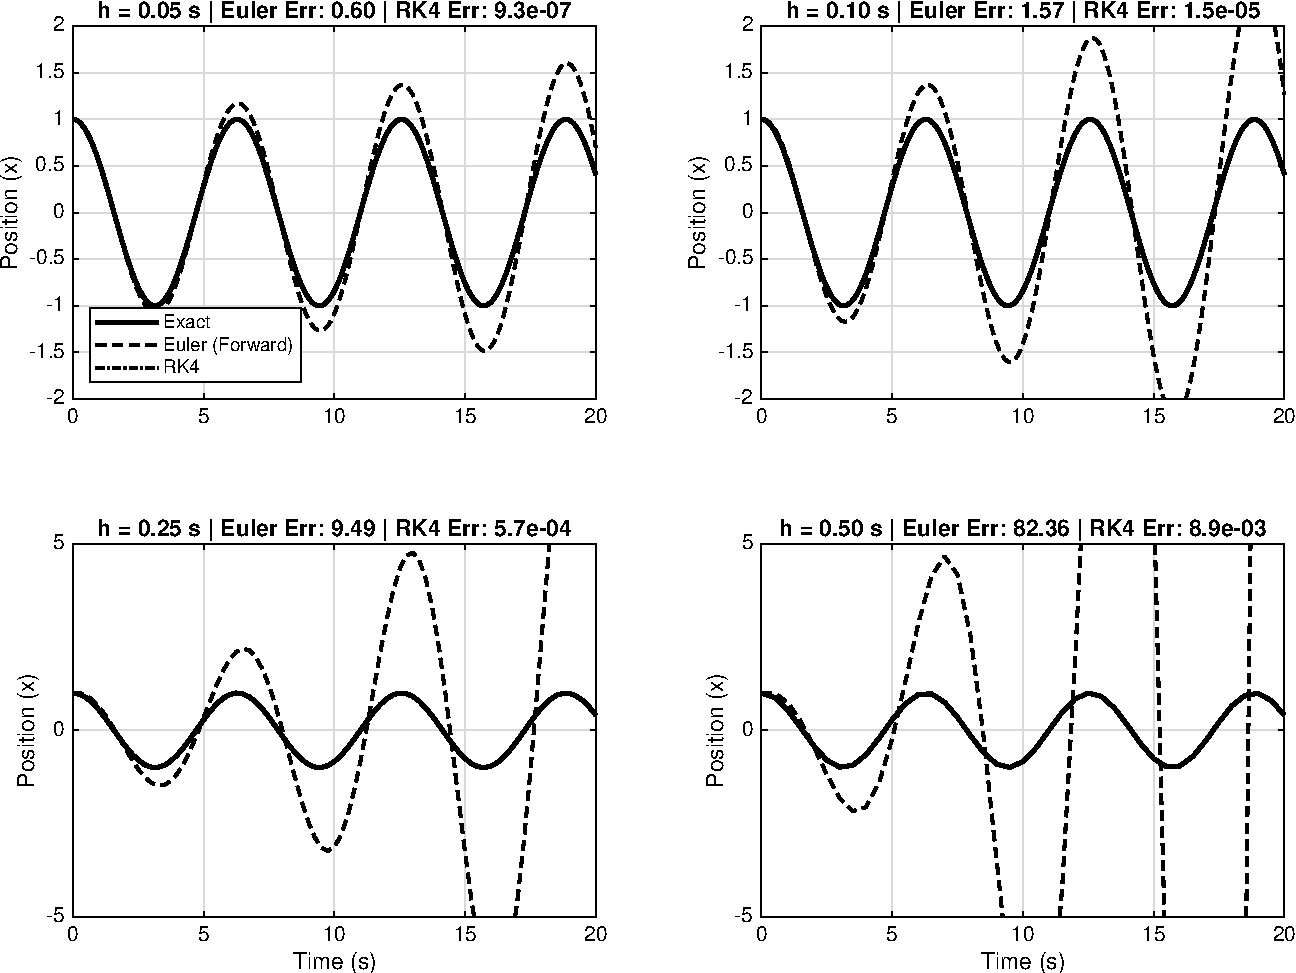
\includegraphics[width=0.6\linewidth]{RK4_vs_euler.pdf}
\end{center}
\end{frame}

\section{Stability of discrete-time systems}

\begin{frame}{Discrete-time stability condition}
For the discrete-time system
\[
x_{k+1}=A_d x_k,
\]
the equilibrium at the origin is asymptotically stable if and only if every eigenvalue of \(A_d\) lies strictly inside the unit circle:
\[
|\lambda_i(A_d)|<1,\qquad \forall i.
\]

\begin{alertbox}{Discrete-time stability test}
Inside unit circle \(\Rightarrow\) asymptotically stable. \\
On unit circle \(\Rightarrow\) marginal behaviour possible. \\
Outside unit circle \(\Rightarrow\) unstable.
\end{alertbox}
\end{frame}

\begin{frame}{Geometric interpretation in the \(z\)-plane}
\begin{itemize}
  \item Stable eigenvalues lie \emph{inside} the unit circle.
  \item Unstable eigenvalues lie \emph{outside}.
  \item Marginally stable eigenvalues lie \emph{on} the unit circle.
\end{itemize}

\begin{center}
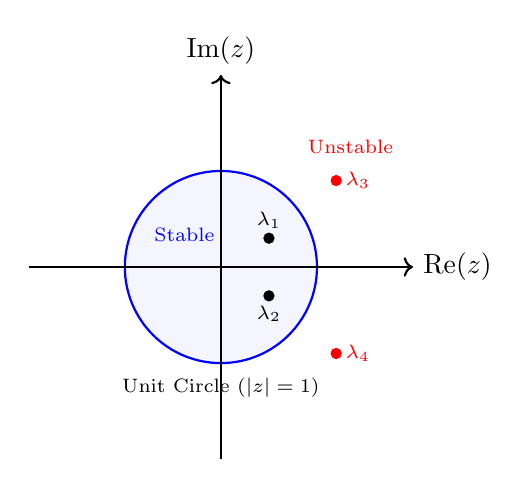
\begin{tikzpicture}[scale=1.22]
  \draw[thick, blue, fill=blue!4] (0,0) circle (1cm);
  \node[blue] at (-0.38,0.34) {\scriptsize Stable};
  \node [red] at (1.35, 1.25) {\scriptsize Unstable};

  \filldraw[black] (0.5, 0.3) circle (1.5pt) node[above] {\scriptsize $\lambda_1$};
  \filldraw[black] (0.5, -0.3) circle (1.5pt) node[below] {\scriptsize $\lambda_2$};
  \filldraw[red] (1.2, 0.9) circle (1.5pt) node[right] {\scriptsize $\lambda_3$};
  \filldraw[red] (1.2, -0.9) circle (1.5pt) node[right] {\scriptsize $\lambda_4$};

  \node[anchor=north] at (0,-1.05) {\scriptsize Unit Circle (\(|z|=1\))};
  \draw[->, thick] (-2,0) -- (2,0) node[right] {Re(\(z\))};
  \draw[->, thick] (0,-2) -- (0,2) node[above] {Im(\(z\))};
\end{tikzpicture}
\end{center}
\end{frame}

\begin{frame}{Continuous-time vs discrete-time stability}
The mapping between continuous-time poles and discrete-time poles is
\[
z=e^{sT},
\]
where \(T\) is the sampling period.

Consequences:
\begin{itemize}
  \item left half-plane in \(s\) maps inside the unit circle in \(z\),
  \item the imaginary axis maps to the unit circle,
  \item the right half-plane maps outside the unit circle.
\end{itemize}

This is why continuous-time stability and discrete-time stability use different geometric tests.
\end{frame}

\begin{frame}{Lyapunov stability in discrete time}
Consider
\[
x_{k+1}=Ax_k.
\]

Define the quadratic candidate
\[
V(x_k)=x_k\T P x_k,
\qquad P\succ 0.
\]

We want the ``energy'' to decrease:
\[
V(x_{k+1})-V(x_k)<0.
\]

Substituting the dynamics,
\begin{align*}
V(x_{k+1})-V(x_k)
&=(Ax_k)\T P(Ax_k)-x_k\T Px_k\\
&=x_k\T (A\T P A - P)x_k.
\end{align*}
\end{frame}

\begin{frame}{The Stein equation}
\begin{alertbox}{Discrete Lyapunov theorem}
The system \(x_{k+1}=Ax_k\) is asymptotically stable if and only if, for any \(Q\succ 0\), there exists a unique \(P\succ 0\) satisfying
\[
A\T P A - P = -Q.
\]
\end{alertbox}

This equation is known as the \textbf{discrete Lyapunov equation} or \textbf{Stein equation}.
\end{frame}

\begin{frame}{Connection to LQR and optimal control}
The Lyapunov viewpoint is fundamental in modern control.

\begin{itemize}
  \item In stability analysis, we seek a function \(V(x)\) that decreases.
  \item In LQR, we shape the closed-loop dynamics so that a quadratic cost and a quadratic Lyapunov function are aligned.
  \item In MPC, we repeatedly optimise future behaviour using the prediction model and a cost function that is strongly connected to these same energy ideas.
\end{itemize}

\begin{notebox}{Conceptual bridge}
State-space modelling \(\rightarrow\) prediction \(\rightarrow\) optimisation \(\rightarrow\) stability.
\end{notebox}
\end{frame}

\section{Key takeaways}

\begin{frame}{Key takeaways}
\begin{itemize}
  \item State-space models describe dynamics through internal variables called states.
  \item Physically meaningful states usually arise from stored energy and configuration variables.
  \item Nonlinear models are often linearised locally around an equilibrium or operating point.
  \item Continuous-time LTI systems can be discretised exactly using the matrix exponential.
  \item Under ZOH, the forced continuous-time model \(\dot{x}=Ax+Bu\) becomes
  \[
  x_{k+1}=A_d x_k + B_d u_k.
  \]
  \item Nonlinear systems usually require approximate numerical integration; RK4 is typically far better than Forward Euler.
  \item Discrete-time stability is characterised by the unit circle.
\end{itemize}
\end{frame}

\begin{frame}{Bridge to the next MPC developments}
From this point onwards, the state-space model becomes the predictive engine inside MPC:
\begin{itemize}
  \item the measured or estimated state \(x_k\) becomes the starting point,
  \item the discrete-time model predicts future trajectories,
  \item constraints are imposed on those future trajectories,
  \item optimisation chooses the best future input sequence.
\end{itemize}

\begin{center}
\textbf{Model + prediction + optimisation = MPC.}
\end{center}
\end{frame}

\end{document}
